\defcitealias{ali_et_al2015}{A15}
\newcommand{\upperlims}{$(1440$ mK$)^{2}$, $(1850$ mK$)^{2}$, $(290$ mK$)^{2}$, $(190$ mK$)^{2}$, $(360$ mK$)^{2}$, $(290$ mK$)^{2}$ at redshifts $z=10.87,\ 9.93,\ 8.68,\ 8.37,\  8.13,$ and $7.48$, respectively}
\newcommand{\hMpci}{h\ {\rm Mpc}^{-1}}

\chapter{PAPER-64 Revised Results}
\label{c.PSA64_results}

\section{Introduction}

Through the re-analysis described in Chapter \ref{c.PSA64}, signal loss (the
unintentional removal of the target cosmological signal) in the empirical covariance
inversion method was discovered \citep{ali_et_al2018}. More specifically, in \citetalias{ali_et_al2015} this signal loss resulted from the use of empirically estimated covariance
matrices as a weighting matrix in the Quadratic Estimator (QE)
during power spectrum estimation.
An empirically estimated covariance matrix contains
terms related to the data, and this dependence induces higher order (i.e., non-quadratic) terms in a QE.
Applying the Optimal Quadratic Estimator (OQE) normalization despite these terms then gives the
wrong power level (i.e., signal loss). This effect is described
more thoroughly in Chapter \ref{c.PSA64}.
Chapter \ref{c.PSA64} also describes how the amount of underestimated signal loss
in the \citetalias{ali_et_al2015} analysis was further obfuscated by similarly underestimated uncertainties (from both analytic noise estimates and bootstrapped error bars). While Chapter \ref{c.PSA64} presents a detailed look
at the origin of these issues, it does not deliver a revised analysis for the same data. In this chapter we present revised limits on the 21\,cm power spectrum using an independently developed pipeline which conservatively has had many steps removed in light of the issues discovered (see Figure \ref{fig:pipeline_compare}).

\begin{figure*}[tp]
\begin{center}
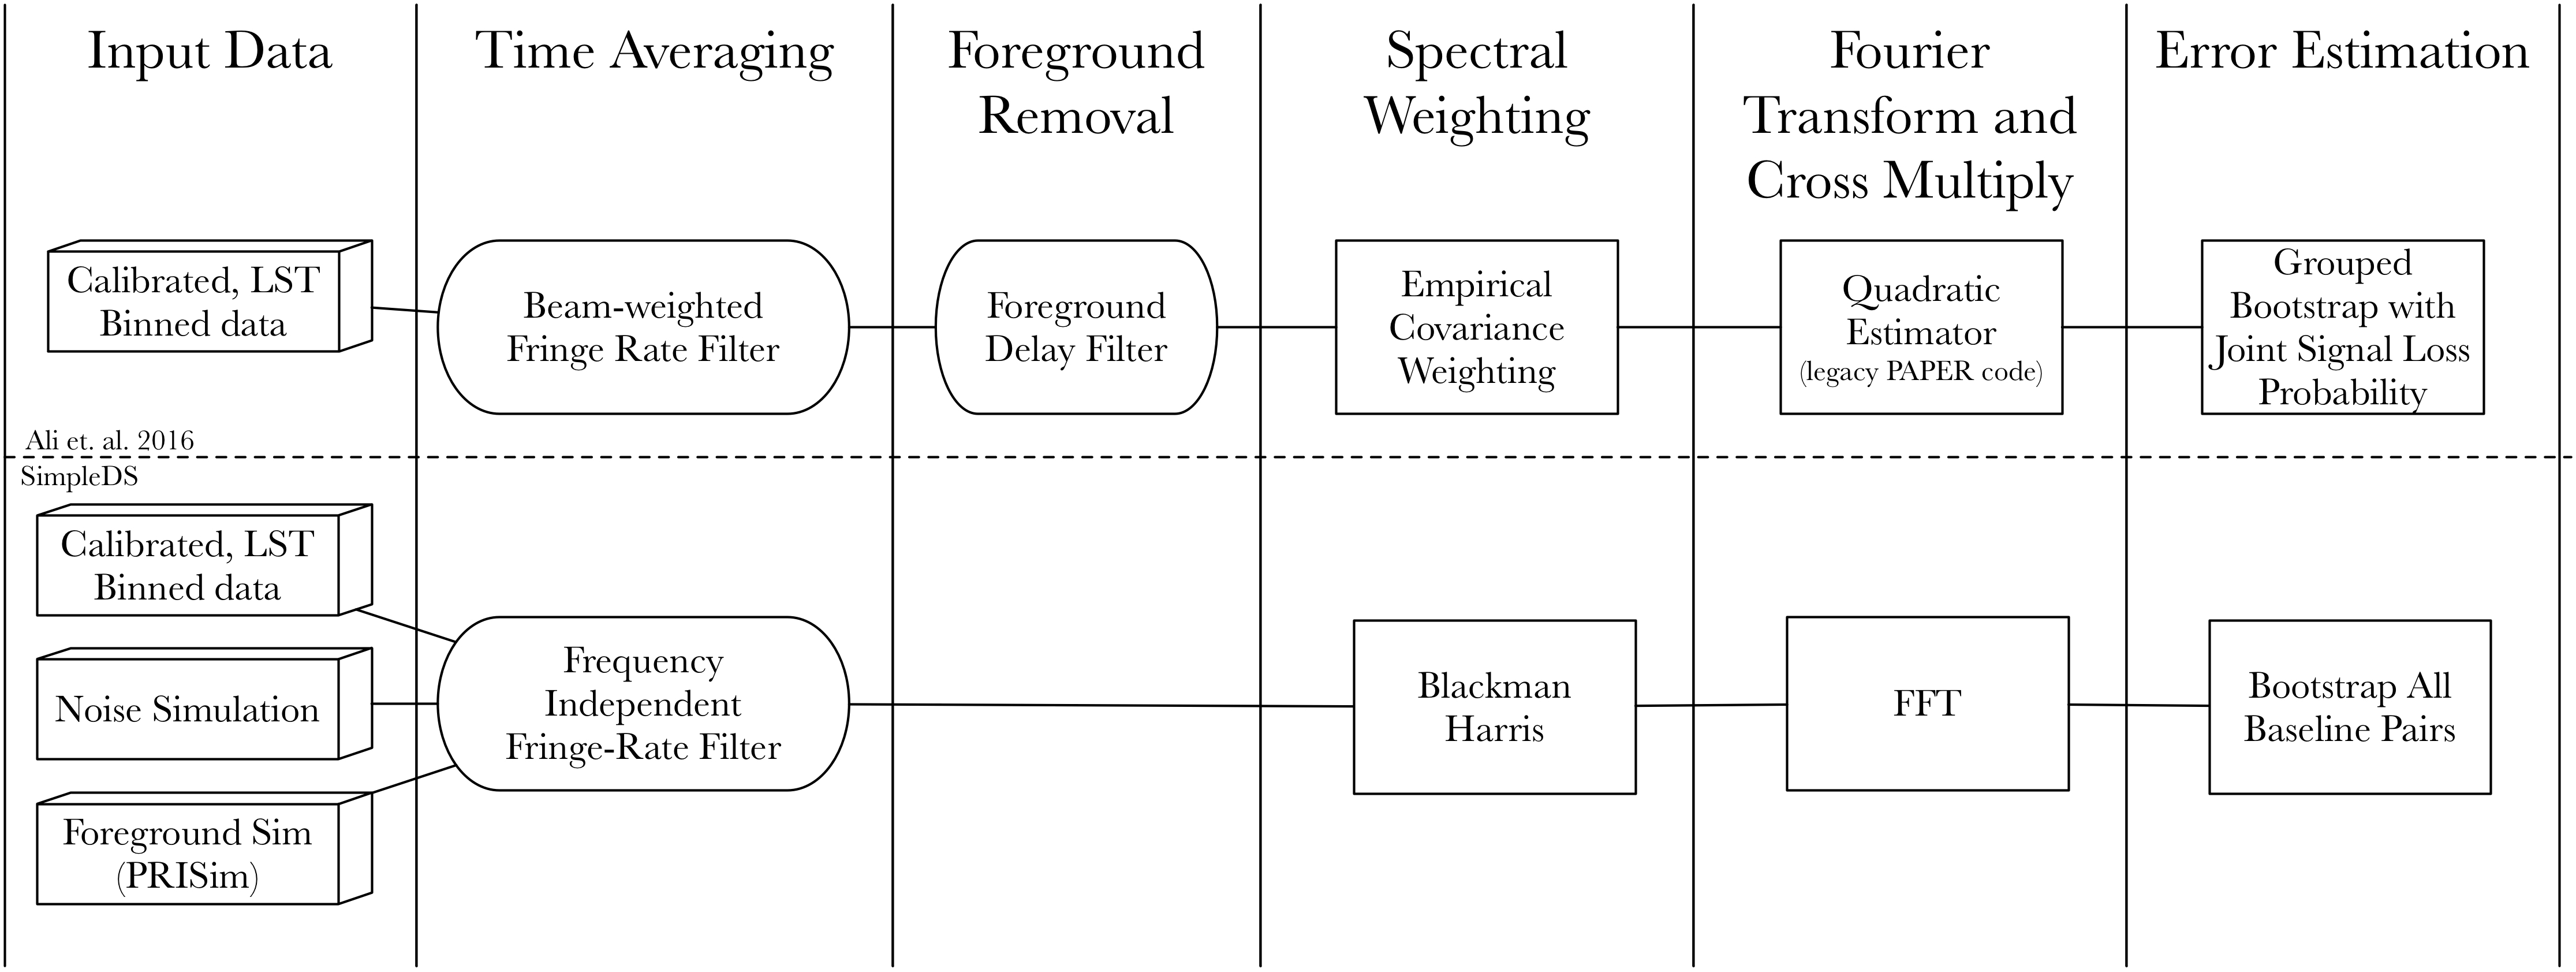
\includegraphics[width=\textwidth]{plots/simpleDS_pipeline_compare.jpg}
\caption{Comparison between the prior PAPER analysis by \citet{ali_et_al2015} and \texttt{simpleDS}'.
Our frequency independent fringe rate filter has a smoother
delay response compared to the one used in
\citet{ali_et_al2015} and
Chapter \ref{c.PSA64} in order to reduce leakage
of foreground power outside the wedge.
Additionally, the delay filter for foreground removal has been
omitted from this analysis to keep the pipeline
as simple as possible. While the foreground removal
technique should not affect cosmological
signals outside the wedge
\citep{parsons_backer2009, parsons_et_al2012b, parsons_et_al2014},
recent works have shown that the use of this filter does
not produce a statistically significant reduction
in power at high delay modes \citep{kerrigan_et_al2018}.
Also, we find that the Fourier-transform used to go from
frequency to delay is not dynamic range limited
when including foreground signals.
Most importantly, in order to avoid signal loss during power spectrum
estimation, we use a uniformly weighted
Fast Fourier-Tranform (FFT) estimator instead of the
empirical inverse covariance weighted OQE used in
previous PAPER analyses.}
\label{fig:pipeline_compare}
\end{center}
\end{figure*}

Specifically, we aim to make improvements in two areas. First, we use the
independently developed pipeline \texttt{simpleDS}\footnote{\url{github.com/mkolopanis/simpleDS}} which has minimal cross common code with the original PAPER pipeline built for \citetalias{ali_et_al2015} and
extended by Chapter \ref{c.PSA64}.
 Second, this analysis reduces the number of pipeline steps.  The basic concept of the delay spectrum
is retained, with a power spectrum measurement coming from each type of baseline; however several steps have been removed and others replaced. In particular, while the re-analysis described in Chapter \ref{c.PSA64} focuses almost exclusively on
the final power spectrum estimation stage, here the intermediate stages (like foreground filtering) have been re-examined.

We expand the subset of data analyzed in Chapter \ref{c.PSA64} to the full PAPER-64 dataset as used in \citetalias{ali_et_al2015} in order to make our revised power spectrum analysis. Data collection and processing steps prior to LST-binning remain identical to previous analyses (Chapters \ref{sec:PSA64_observations} and \ref{sec:PSA64_processing}). We analyze the same three 30\,m baselines as in \citetalias{ali_et_al2015} and form estimates for six independent redshift bands. In selecting our bands, we note that a practical limitation in selection
comes from a desire to avoid including channels with significant RFI flagging.
Bands with the most continuous spectral sampling span the redshift range $7.5$ to $11$, and we select redshift ranges that are approximately coeval, i.e., bandwidths over which limited evolution of the 21\,cm signal is expected.
Constraints from EDGES \emph{high} suggest that the evolution is probably slower than a $dz$ (total change in
redshift) of 1-2 \citep{monsalve_et_al2017} 
which corresponds to a spectral width of $ 26 $~MHz at frequency 200MHz and 
$12$~MHz at frequency 100MHz.  We adopt a band size of $10$~MHz as a conservative size.

This band size allows us to choose a number of spectral windows with very little to no RFI flagging.  The specific windows chosen here are centered on
$z=10.87,$ $9.93,$ $8.68$, $8.13,$ and $7.48$ ($119.7$, $130.0$, $146.7$, $155.6$, and $167.5$~MHz respectively).
As a validation check, we also include
a reprocessing of the $z=8.37$ bin centered at $151.6~$MHz
which was analyzed in \citetalias{ali_et_al2015} and Chapter \ref{c.PSA64}.
These bands are illustrated visually in Figure~\ref{fig:freq_select}.

\begin{figure*}[t]
\centering
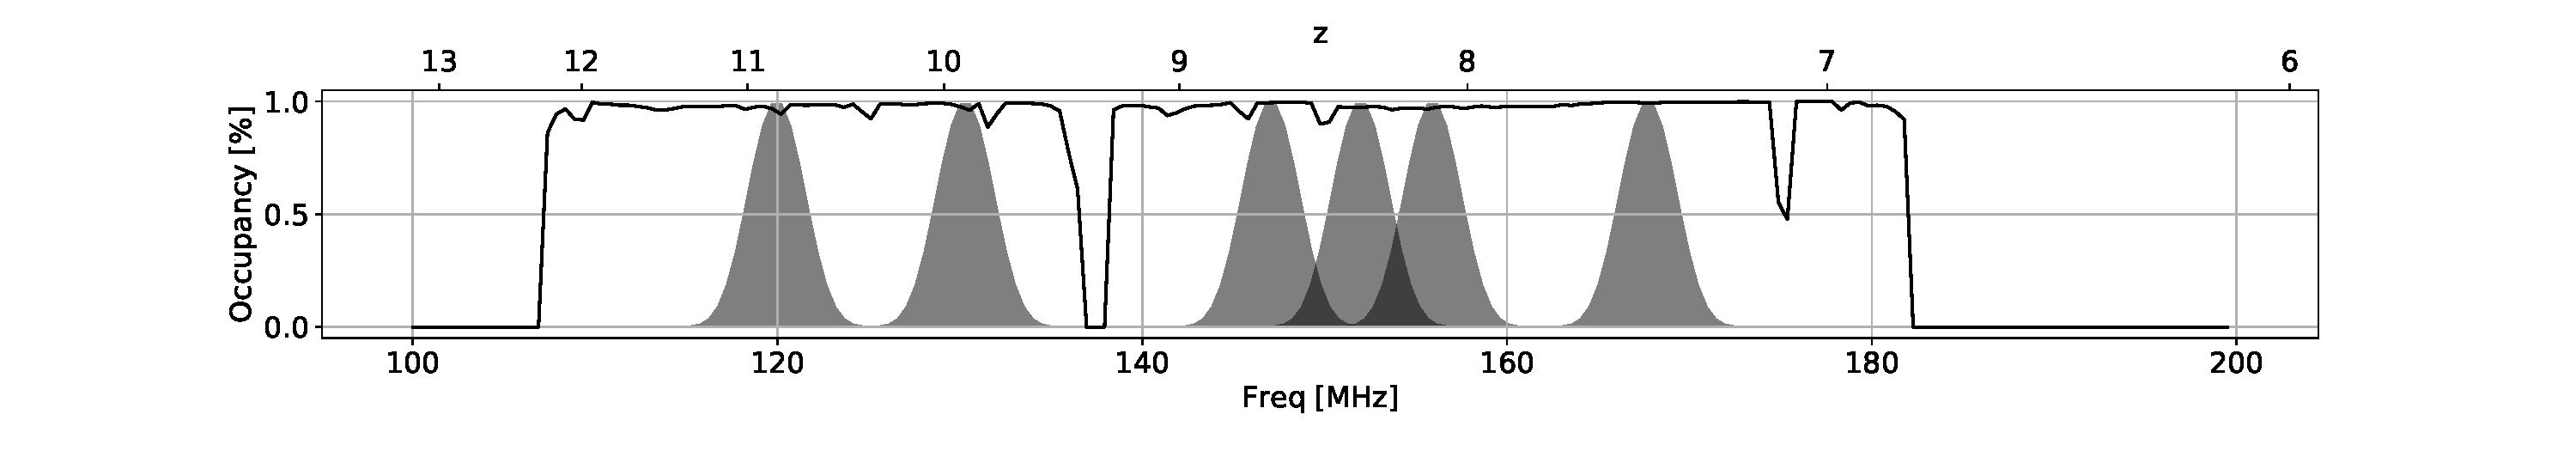
\includegraphics[trim={4cm 0  5cm 0},width=\textwidth]{plots/freq_select_BH.pdf}
\caption{The six frequency bands used in this analysis plotted over the relative number of total binned days in a frequency bin (e.g., the relative fraction of total days used in LST binning).
Redshift bands are denoted by the
Blackman-Harris window functions used during
the Fourier-transform from frequency to delay in order
to reduce foreground leakage to high delays.
All frequency bands used in this analysis have been shown, including the $z=8.37$ ($151.6$\,MHz) band used in \ref{c.PSA64} and \citet{ali_et_al2015}.
This redshift bin is included in order
to properly compare with previous works,
but it is worth noting the information
obtained from this bin is not entirely independent from the two
redshift bins with which it overlaps.
\label{fig:freq_select}}
\end{figure*}

This chapter is organized in three main parts. We first present major differences between the \texttt{simpleDS} pipeline and that of \citetalias{ali_et_al2015}, including an investigation into the redundancy of PAPER-64 which motivated the removal of certain contaminated data prior to power spectrum analysis. Then, we present our multi-redshift power spectrum results supported by a discussion into systematics through the interpretation of jackknife and null tests. Finally, we present 21\,cm upper limits within the context of the broader field. 

\section{A Simplified Pipeline}

In this section we describe the differences in the analysis steps prior to power spectrum estimation
 between this work and \citetalias{ali_et_al2015}, including time-averaging, foreground removal techniques, and flagging on redundant baselines (see Figure~\ref{fig:pipeline_compare}).

\begin{figure}
\centering
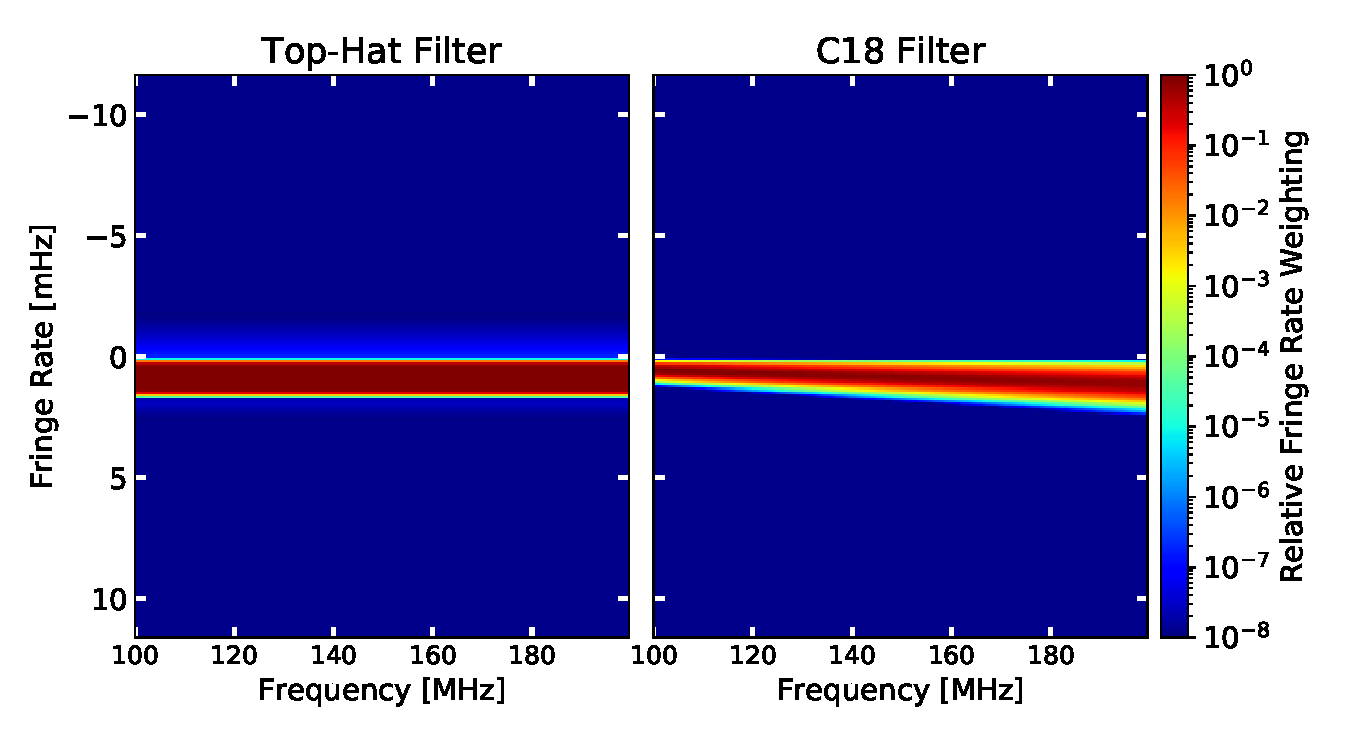
\includegraphics[width=.85\textwidth]{plots/frf_comparison_waterfall.pdf}
\caption{A comparison of the Top-Hat fringe-rate filter (TH, left) and the filter used in Chapter \ref{c.PSA64} (right) in the fringe-rate, frequency domain.
The Chapter \ref{c.PSA64} filter (and the \citet{ali_et_al2015} filter)
varies with frequency and this spectral
variation can cause additional structure
when performing a delay transform of the visibilities. In the interest of simplicity
in this analysis, we choose to perform time-averaging with the
Top-Hat filter.
}\label{fig:FRF_response}
\end{figure}

\begin{figure}[tp]
\centering
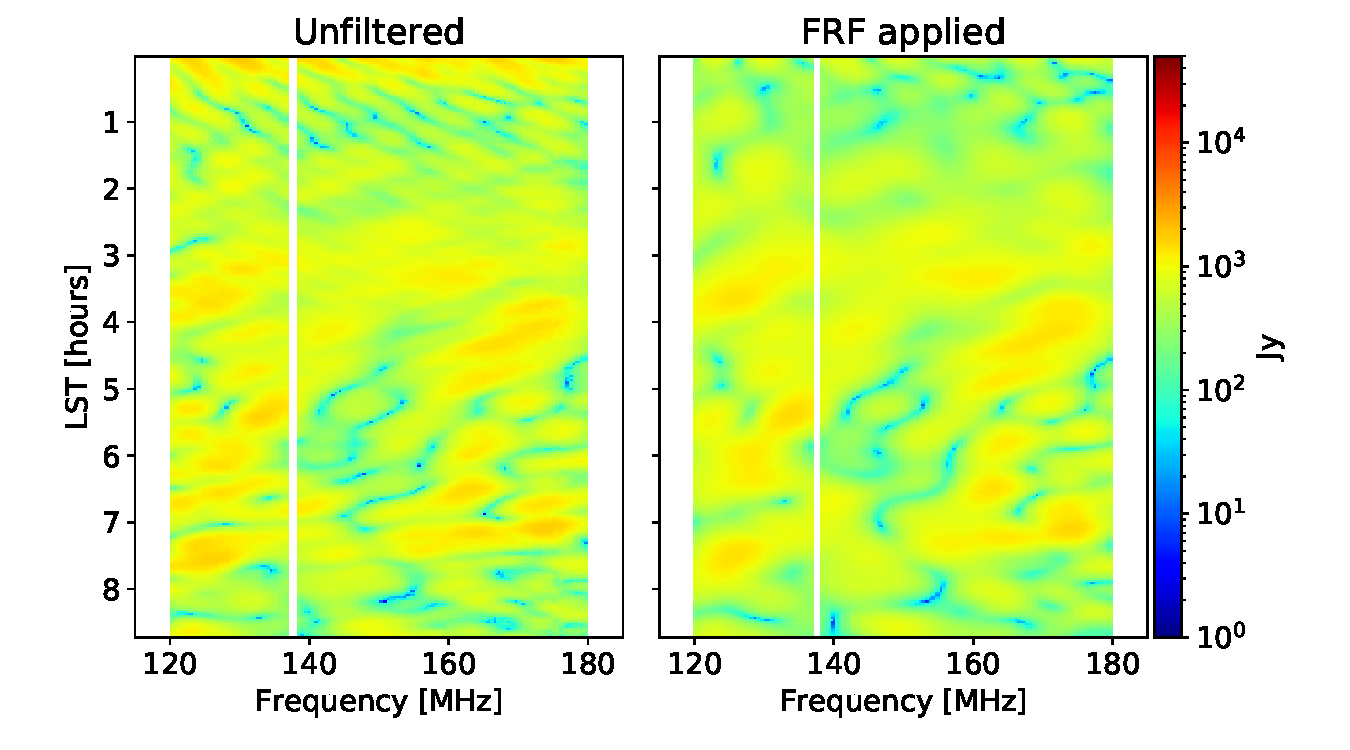
\includegraphics[width=.85\textwidth]{plots/data_bl_waterfalls.pdf}
\caption{LST and frequency waterfalls of a representative
baseline taken from the even LST binned set before (left)
and after (right) application of the Top-Hat FRF.
The baseline illustrated is the antenna pair (1,4). The application of the fringe-rate filter removes very fast
fringe modes but preserves the structure of sky-like
modes.}
\label{fig:waterfalls}
\end{figure}

\subsection{Time-averaging}

The LST-binned PAPER-64 data have been averaged into $43$~s bins, a timescale
which is short compared to the $\sim$3500~s fringe coherence time of 30\,m baselines.
Here, as in past PAPER analyses, we choose to perform time-averaging by convolving the time stream with a windowing function.
This function is defined as a filter in fringe-rate space
(the Fourier dual to time) which can be tuned to maximize sensitivity to sky-like modes and exclude slowly varying systematics.
\cite{parsons_backer2009} show that
a fringe-rate corresponds to sky-like rates of motion which map geometrically to
a great circle on the sky.
\cite{parsons_et_al2016} then show that a fringe-rate filter (FRF) can be defined with weights corresponding
to the instrument's primary beam power integrated along the line of constant fringe-rate. Applying an FRF with this weighting provides the longest possible coherent integration in time for a baseline of a given length.

Previous PAPER analyses have used variations on such a filter.  \citetalias{ali_et_al2015}
formed the beam-weighted filter, fit a Gaussian
in fringe-rate space, and then artificially increased
the width of the Gaussian
to provide easy parameterization across the PAPER
bandpass and decrease the effective integration time.
A similar Gaussian fit was
also used and discussed in the PAPER-64 case study in Chapter \ref{c.PSA64},
but the width of the fit was not increased in that
analysis.

However, as can be seen in the right panel of Figure \ref{fig:FRF_response}, this filter is frequency dependent.
In particular, the maximum fringe-rate range probed by a baseline increases linearly with frequency.
This spectral dependence may introduce additional structure during the delay transform; further investigation is needed to find the best approach for mitigating this effect.
We also recall that the use of these ``aggressive" fringe-rate filters is shown to contribute to signal loss
(Chapter \ref{sec:toymodel_frf}).

Therefore, as a simplification to avoid potential signal loss
and reduce contamination of high delay modes,
we adopt a Top-Hat filter (left panel, Figure \ref{fig:FRF_response})
that weights all fringe-rates evenly across frequency, similar to the filter used in \citet{parsons_et_al2012b}.
The maximum fringe-rate passed by our filter is set
by the highest frequency
included in the data set; the lowest fringe-rate is chosen to exclude known common mode signals with zero fringe
rates.

Common mode signals are those which vary on time scales longer than would be expected from an ideal interferometer \citep{ali_et_al2015}.
Such common modes were previously referred to as
	``crosstalk'' --- however, these signals may not
	necessarily result from signals observed in one antenna and leaked to another
	(a time-delayed sky signal) but rather any time-independent signal which is observed by all antennas. We exclude common mode signals here by setting the minimum fringe-rate included in the filter to $3.5\times10^{-5}$~Hz; this
excludes all modes with periods longer than $\sim$45 minutes.

%Suppressing slowly or negatively fringing sources will suppress sources with 
%elevations at or below the South Celestial
%Pole. These modes are generally
%low in the $\sim 45\arcdeg$ PAPER primary beam.
%When applying this filter to our foreground simulation,
% the total simulated flux density is observed to decrease by $\sim 3\%$.

Waterfalls of a representative baseline
before and after the application of the
fringe-rate filer are shown in Figure~\ref{fig:waterfalls}.
The application of the fringe-rate filter removes very fast
fringe modes but preserves the structure of Eastward moving sky-like modes.

\subsection{Foreground Removal}\label{sec:wida}

To mitigate foreground contamination during
power spectrum estimation, PAPER analyses have used
a wide-band iterative deconvolution algorithm (WIDA),
often referred to as a ``clean-like'' iterative
deconvolution algorithm. This algorithm relies on the
underlying mathematics of CLEAN as described in
\citet{hogbom1974} to remove delay components from
PAPER data inside of some range of delays.
This type of deconvolution and its specific
application to radio data is described in \citet{parsons_backer2009}.
The WIDA was used in \citet{parsons_et_al2012b,parsons_et_al2014,jacobs_et_al2015}, \citetalias{ali_et_al2015}, \citet{kerrigan_et_al2018}, and Chapter \ref{c.PSA64}.

We choose to omit this filtering technique in our simplified analysis. While the technique should not
affect cosmological signals outside the user-defined
range of delays to clean (\citealt{parsons_backer2009, parsons_et_al2012b, parsons_et_al2014}, and explored further in \citealt{kerrigan_et_al2018}),
recent works have also shown that the use of this filter does not produce
statistically significant reduction of power at
high delay modes \citep{kerrigan_et_al2018}.
Since our analysis aims to focus on upper limits set
at high delay modes, we omit this step in the interest
of simplicity. Even without any attempt to remove foregrounds from the
visibility data, we find that our delay transform used to estimate
the cosmological power spectrum is not limited by the inherent
dynamic range of the transform.

\subsection{Flagging on Redundancy}
\label{sec:redundancy}

\begin{figure*}[tp]
\centering
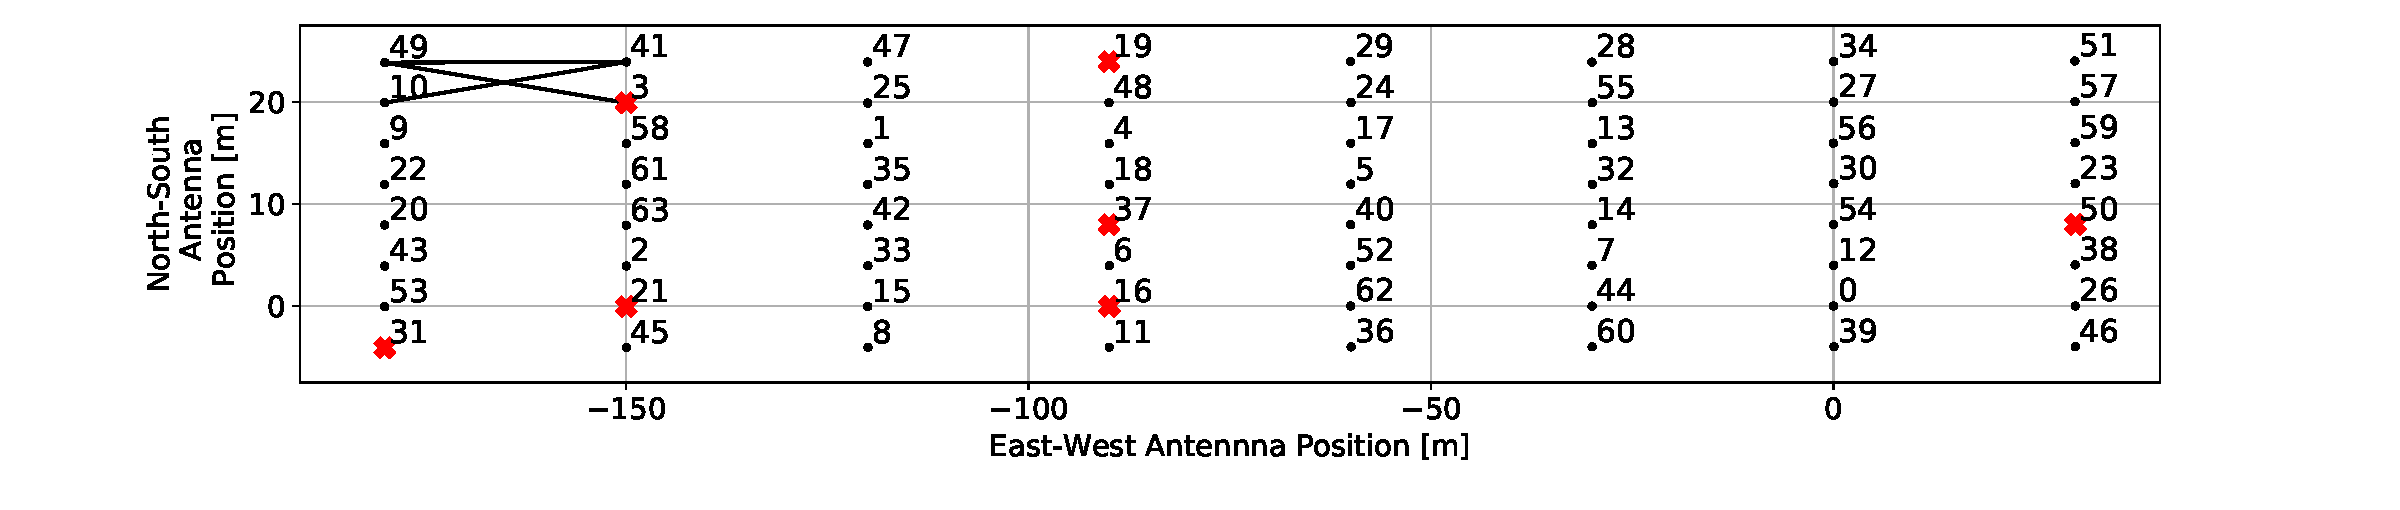
\includegraphics[trim={3cm 0  4cm 0},width=\textwidth]{plots/psa64_antpos_flagged.pdf}
\caption{The antenna positions of PAPER-64.
Highlighted are the three baseline types used in this analysis.
These baselines consist of East-West baselines from adjacent
antenna columns with no row separation
(e.g., 49-41, 1-4, 0-26),
baselines with one column separation and one positive Northward
row separation (e.g., 10-41, 1-48, 0-38),
and baselines with one column separation
and one negative Northward row separation
(e.g., 49-3, 1-18, 0-46). A red `x' denotes antennas which have been flagged from the analysis. Reasons for
flagging include previously known spectral instability (19, 37, and 50), low number of counts in LST binning (3 and 16), and suspected non-redundant information (21 and 31).} \label{fig:ant_pos}
\end{figure*}

\begin{figure}[tp]
	\centering
	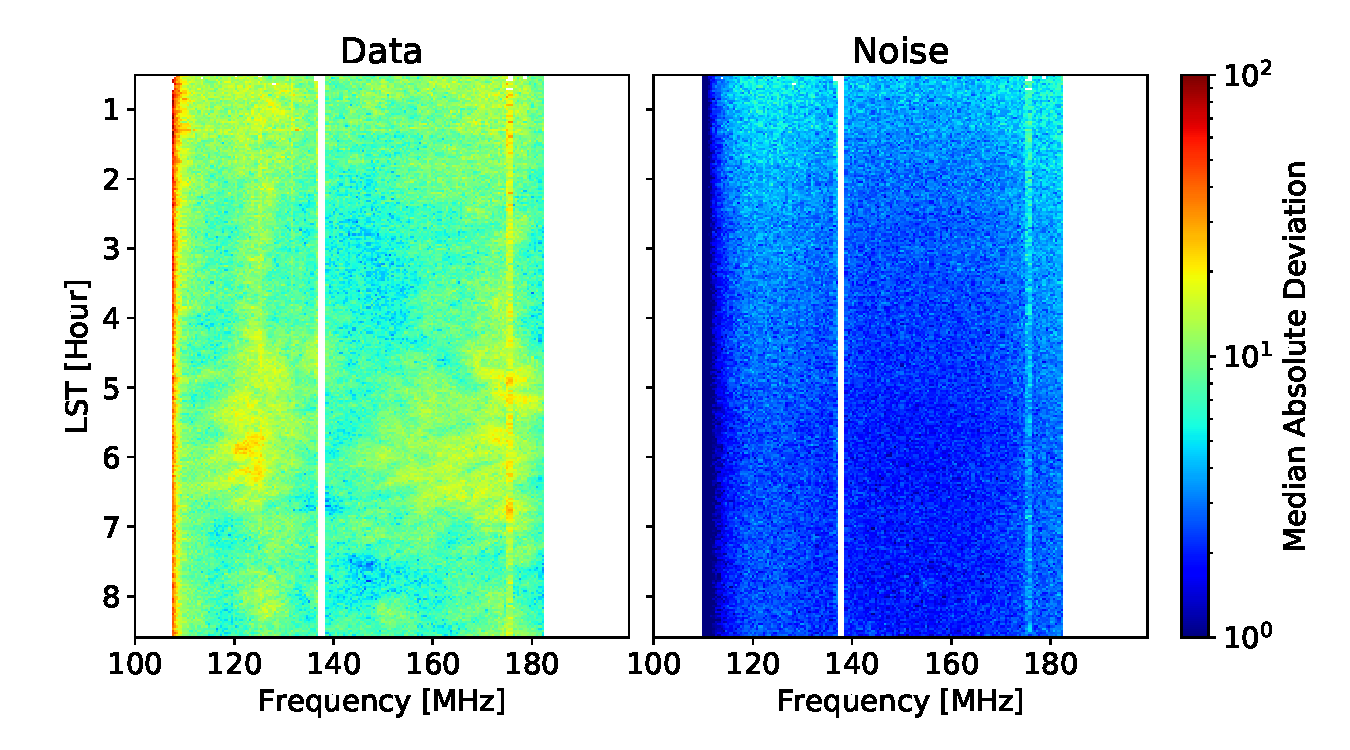
\includegraphics[width=.85\textwidth]{plots/data_noise_mad_O.pdf}
	\caption{A representative Median Absolute Deviation (MAD) for both data (left)
		and noise simulation (right) computed for each time and frequency observed by
		PAPER in the LST range $00^{h}30^{m}00^{s} - 08^{h}36^{m}00^{s}$.
    The data shown here corresponds to
		strictly 30\,m East-West baselines.
		For perfectly redundant sky measurements the individual
		baseline measurements will only differ by thermal noise.
		The large amplitude of deviations observed here
		illustrates that there is a significant
		amount of non-redundant information in the data.}\label{fig:mad}
\end{figure}

We have described how we simplified both the time-averaging and foreground filtering steps of our pipeline. Finally, before estimating the power spectrum of our data, we conduct statistical tests on our observations to determine the degree to which
our baselines are redundant.
We do this because the per-baseline delay spectrum
estimation technique described in \citet{parsons_et_al2012b}
can be averaged across all baseline cross-multiples only for
perfectly redundant baselines. While it is unrealistic to assume
the PAPER baselines are perfectly redundant, this analysis can
help identify extreme outliers which should not be used in
power spectrum estimation.

In Figure \ref{fig:ant_pos}, we show the 8 x 8 antenna configuration used in the PAPER-64 deployment, which was chosen to increase power spectrum sensitivity through having many copies of the same baseline (i.e., redundant observations). Each of the three baseline vectors shown  (which we use for our revised power spectrum analysis in this chapter) are
sampled many times across the grid-like array. Rather than average
baselines together (as was done in previous PAPER analyses for computational simplicity)
we cross-multiply all redundant pairs and then bootstrap average for
an estimate of variance. Our bootstrapping procedure was described in more detail in Chapter \ref{sec:Boot}.

A first test of the array's redundancy is to compare the measured variation between baselines
with that expected due to thermal noise, using Equation \eqref{eq:sense}
to generate noise for each time and frequency for each baseline.
As a measure of variance between baselines we take the Median Absolute Deviation
(MAD) of the visibility amplitude across redundant baselines
for each frequency and time, defined as
\begin{equation}
\text{MAD}(t,\nu) = median\left(\left| \left|V_{i,j}(t,\nu)\right|  - median \left(V(t,\nu)\right) \right|\right)\label{eqn:mad}
\end{equation}
where the median visibility amplitude is taken
at each time and frequency across the redundant baseline group.

The MAD for both data and our noise simulation is shown in  Figure~\ref{fig:mad}.
For perfectly redundant sky measurements the individual
baseline measurements will only differ by thermal noise.
We see that some measurements have a MAD consistent with thermal noise ---
however the larger deviations observed at other frequencies and times
illustrates a significant amount of non-redundant information in the data.

We then use the MAD to estimate the significance of each baseline's
deviation from the median baseline measurement using the modified z-score ($ M_{z}(t,\nu) $) defined as
\begin{equation}
M_{z}(t,\nu) = 0.6745\frac{\left|V_{i,j}(t,\nu) - median \left(V(t,\nu)
	\right)\right|}{MAD} \label{eqn:zscore}
\end{equation}
which can be thought of as the number of standard deviations
away from the median each data point is.
The $ 0.6745 $ scaling factor is introduced to normalize the
modified z-score for a large number of samples \citep{Iglewicz_and_hoaglin}.

The waterfalls of z-scores (in time and frequency) are averaged in LST
and a maximum is taken along the frequency dimension to find a single
worst case modified z-score for each baseline.
The histogram of these z-scores for every baseline in this analysis is shown in Figure~\ref{fig:mod_z_score_avg}.
As suggested in \citet{Iglewicz_and_hoaglin},
any baseline with a modified z-score of at least $ 3.5 $ is identified as a potential outlier.

Using this metric, only the baseline $ (21,31)  $
is identified as an outlier. With only one outlier, it is difficult
to tell if this deviation is due
to a single defective antenna or the physical baseline.
We take the most conservative approach and flag
both antennas 21 and 31 from all remaining analysis.
Although no other baselines qualify as outliers,
the existence of scores above 2 in general
indicates an amount of non-redundancy
inconsistent with thermal noise from the baselines in this analysis and may affect
the interpretation of our final
power spectrum estimates.

\begin{figure}[tp]
	\centering
	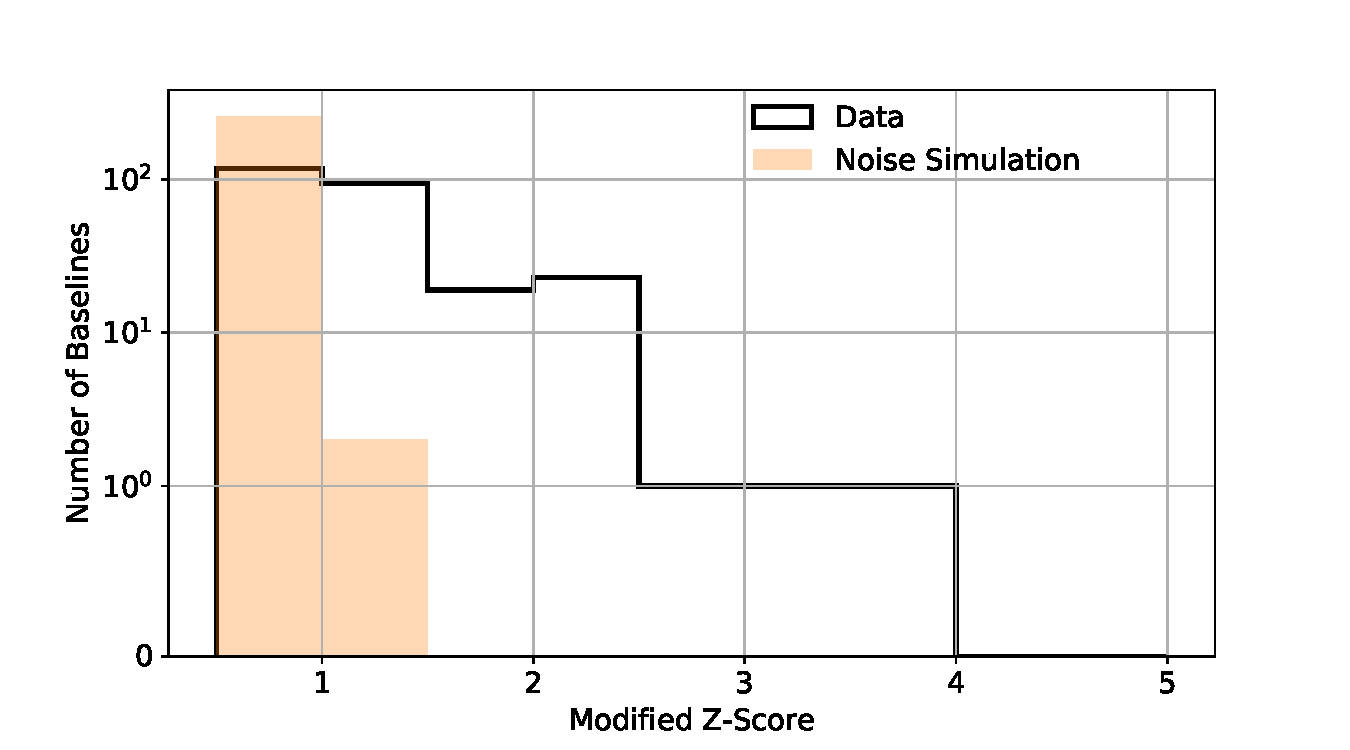
\includegraphics[width=.85\textwidth]{plots/zscore_hist.pdf}
	\caption{A histogram of modified z-scores of data (black) 
		and input noise simulation (orange) suggests that a cut on baselines
		with z-score larger than 3.5 will safely avoid statistically outliers (e.g., non-redundant baselines). This is consistent with the
		recommendation from \cite{Iglewicz_and_hoaglin}. Using this metric,
		only the baseline (21,31) is a statistically significant outlier. Since it is unclear which of the two antennas may be contributing to this non-redundancy we flag both antennas in all further analysis.} %The two noise data points in the bin [1,1.5) correspond to baselines (21,31) and (31, 45), both of which have large modified z-scores in the data case.}
\label{fig:mod_z_score_avg}
\end{figure}

\section{Multi-Redshift Power Spectrum Results}\label{sec:pspec_results}

In this section, we present power spectrum results for all six of our redshift bands. We show three principal products: our observed data, a simulated foreground observation, and a noise-only simulation. Broadly speaking, the simulated foreground observation is created using the simulator PRISim \citep{Thyagarajan_et_al2015a, Thyagarajan_et_al2015b}, which performs a full-sky visibility calculation matching the observing parameters of PAPER's LST-binned data set. For more details about the construction and accuracy of the sky simulation, we refer the reader to Kolopanis et al. (\textit{in prep.}). Power spectra of the other two products, data and noise-only, are produced similarly to those in Chapter \ref{c.PSA64}, but with an unweighted, non-lossy estimator.

\begin{figure*}[tp]
\centering
\includegraphics[width=\textwidth]{plots/pspec_pk_vs_sim.pdf}
\caption{Power spectrum estimates computed for
the observed data (black), simulated noise (orange), and simulated foreground observation (blue).
Error bars on data points are the bootstrapped $2\sigma$ uncertainty.
The solid green line indicates the theoretical thermal
noise estimate for each redshift bin, and the dashed
green line includes a modeled foreground error (Kolopanis et al. (\textit{in prep.})).
Gray shaded regions are the foreground dependent uncertainties plotted around each data point.
The vertical black dotted lines indicate the horizon/wedge/light travel time for a 30~m
baseline. We find that the simulated noise is consistent with
the theoretical thermal noise predictions (orange vs. solid green).
At delay $\tau = 0$\,ns, both the data and foreground simulation
show good agreement in the total power observed;
generally, the power at all delays inside the horizon agrees between the two simulations within a factor of $ \sim5 $. The simulated data set also shows some
power leakage outside the horizon,
consistent with the power observed by PAPER out to $ \sim 400$\,ns. The PAPER data also show numerous statistically significant detections beyond 400\,ns, however, which are not predicted by the foreground simulation.
To investigate the origin of these signals, multiple jackknives and null tests are performed.}
\label{fig:pspec_vs_sim}
\end{figure*}

Figure~\ref{fig:pspec_vs_sim} shows the delay power spectrum estimates for our three products: the observed data (black),
the PRISim simulated foreground observation (blue), and the noise-only simulation (orange).
Within delay modes between $ \sim\pm 400 $~ns, both the observed and simulated data illustrate
similar shapes. This suggests that the statistically significant detections of power
observed in PAPER immediately outside the horizon limits
are consistent with foreground signals (as suggested by the study of foreground subtraction applied to PAPER data in \citealt{kerrigan_et_al2018}). At larger delays, however, the PAPER power spectra are a mix of statistically significant detections and null results. The most statistically significant detections at high delays are seen to occur at the lowest frequencies. In the next few subsections, we present several analyses designed to help determine the cause of the statistically significant detections at high delays seen in the PAPER observations.

\begin{figure*}[tp]
\centering
\includegraphics[width=\textwidth]{plots/pspec_real_imag.pdf}
\caption{The real (black) and imaginary (red) components of the
power spectrum. The red shaded region is the 
foreground dependent theoretical error drawn around the 
imaginary components; all other lines are the same as in Figure~\ref{fig:pspec_vs_sim}. There are statistically significant imaginary components at
$ |\tau| < 400 $~ns, generally at a power level
which is $ \sim 20\% $ of the real components at the same delay.
This may result from non-redundancies in calibration or baseline orientation. At delay modes $ |\tau| > 400 $~ns, the imaginary
component of the power spectrum displays comparable power to the 
real part. This is especially prominent in, but not isolated to, the two lowest redshift bins. The statistically significant imaginary power is indicative of some non-redundant information 
during power spectrum estimation, systematic biases introduced during data analysis or calibration, 
or residual contaminants like improperly flagged RFI.
}
\label{fig:real_imag}
\end{figure*}

\subsection{Investigation of High Delay Detections}

The power spectrum is computed by cross-multiplying
different baseline pairs within redundant baseline groups.
Ideally, this cross-multiplication of complex-valued
delay spectra will result in any sky-like power being confined to the real part in the power spectrum, leaving the imaginary part dominated by noise.
However, effects can leak real sky power into the
imaginary part of the spectrum.
A perfectly calibrated array with non-redundant baselines
--- for example, with slightly different antenna positions ---
will cause two nominally ``redundant'' baselines to have slightly different phases.
The imaginary parts of these cross-multiplied visibilities will therefore not cancel out, and non-zero power will be seen in the imaginary component of the power spectrum estimate.
The same effect would come from a perfectly redundant but imperfectly calibrated array.
%It is also important to note that because of the foreground-dependent error bars derived in Section~\ref{sec:FG_err},
%imaginary power should increase at low delay, though continue to be consistent with zero.
In a sense, the amount of statistically significant power in the imaginary component of the power spectrum, compared to power in the real part, is a measure of the net redundancy and calibration quality of the array.

A comparison of the real and imaginary parts of the power spectrum
is shown in Figure~\ref{fig:real_imag}.
The statistically significant imaginary components at
$ |\tau| < 400 $~ns (red) are generally at a power level
which is $ \sim 20\% $ of the real components (black) at the same delay.
This may result from non-redundancies in calibration or baseline orientation.

At delay modes $ |\tau| > 400 $~ns, the imaginary
component of the power spectrum displays comparable power to the 
real part. This is especially prominent in the two lowest redshift bins, but is observable across the entire band.
The disagreement between the imaginary component (red) and the estimated foreground error (dashed green) is indicative of some non-redundant information, systematic biases introduced by data analysis or calibration steps, or residual contaminants like improperly flagged RFI.

\begin{figure*}[tp]
\centering
\includegraphics[width=\textwidth]{plots/pspec_lst_null_test.pdf}
\caption{Null tests constructed by splitting the LST range ($[00^{h}30^{m}00^{s}, 08^{h}36^{m}00^{s}) $) in half (at $04^{h}30^{m}$), making two
power spectrum estimates and differencing the result. Real (black) and imaginary (red) parts are both shown, along with the null test results
when applied to the simulated data (blue). All noise estimates shown are as described in Figure~\ref{fig:pspec_vs_sim}.
Such a null test should remove
isotropic cosmological signals, leaving behind anything with dependence on sidereal time. Statistically significant detections in the real part suggest power varying across the sky while significant imaginary power suggests a time dependence to phase calibration errors. The observed variations are consistent with the simulation up to delays of 400\,ns.
The detections at higher delay modes indicate a large 
LST dependence which is inconsistent with cosmological power.}
\label{fig:lst_null_test}
\end{figure*}

\begin{figure*}[tp]
\centering
\includegraphics[width=\textwidth]{plots/pspec_even_odd_null_test.pdf}
\caption{Jackknife test constructed by splitting the data set by even and odd Julian day. Plotted here is the difference between the power spectra from these two sets. We use the same color scheme as Figure~\ref{fig:lst_null_test}. While the largest difference in the LST null test
(Figure \ref{fig:lst_null_test}) was on the order of 10\% of the measured value, here differences are less than 1\% at delays less than 400\,ns, and the imaginary points are nearly all consistent with predicted error bars. At delays larger than 400\,ns, statistically significant detections
in the three highest redshift bands are at comparable
levels to the power spectrum values in Figure~\ref{fig:pspec_vs_sim}.
This may be the result of contamination in only one set of the even or odd data (positive value for even, negative values for odd) which are mitigated during the cross-multiplication of these sets during power spectrum estimation.}
\label{fig:even_odd_null_test}
\end{figure*}

\subsection{Null Tests}\label{sec:nulls}

While the presence of imaginary power suggests at least some presence of calibration error or non-redundancy, it does not fully explain the origin of the excess power at delays greater than 400\,ns. Calibration errors, as long as they do not introduce
spectral structure, should not necessarily scatter power to high delays. Null tests --- i.e., differences between
power spectra of different data selections --- can provide hints at the origin of these detections (Chapter \ref{sec:JackknifeOverview}).

For example, differencing the power spectra of two distinct ranges of sidereal time will remove
isotropic cosmological signals but leave behind signals with strong dependence on sidereal time (like foregrounds).
Dividing our data set in half by LST into ranges $ [00^{h}30^{m}00^{s}, 04^{h}30^{m}00^{s}) $
and $ [04^{h}30^{m}00^{s}, 08^{h}36^{m}00^{s}) $ creates two sets of roughly equal sensitivity.
The resulting differenced power spectrum is shown in Figure~\ref{fig:lst_null_test}, along with a matching calculation for the foreground simulation.
The two are broadly consistent at
delays less than 400\,ns, i.e., they have the same sign and a
similar amplitude. Galactic synchrotron emission and bright point sources (like Fornax A
and Pictor A) are the most obvious contenders for strong variability. We also see that the significant power seen in modes well beyond the horizon (for example, the strong positive offset at redshift 9.93 seen in the Figure~\ref{fig:pspec_vs_sim} power spectrum) is reflected in this null test.

Additionally, we see that the imaginary component of the power spectrum null test is comparable to the real component at most delay modes across all redshifts. 
This suggests a sidereal time dependence of phase differences between baselines. In particular, note that the strong bias seen at redshift 9.93 is associated with a strong imaginary bias, implying a phase rotation between baselines. Such an LST dependence of the imaginary component might be expected for non-redundancy (slightly different sky seen by nominally redundant baselines) or repeatable differences in calibration which depend on the sky configuration (for example, one calibration solution when Fornax is transiting and a different one for when Pictor dominates). This kind of variation in redundant calibration with sky flux density was shown in \citet{joseph_et_al2018}. This picture of non-redundancy strengthens the earlier hints provided by the z-score analysis in Section~\ref{sec:redundancy}, which suggested that redundancy was particularly low around $120$-$130$\,MHz (redshifts 9 and 10).

A second easily constructed null test is to difference
power spectra made from only the even and odd binned data sets.
Recall that these sets were constructed by separating even and odd
numbered days during LST-binning. A significant difference in this test would therefore be suggestive of
a variation at the night-to-night level,
as these two sets are otherwise
expected to have identical sky signals
with different realizations of noise.

The resulting even/odd differenced power spectra for each redshift band
are shown in Figure~\ref{fig:even_odd_null_test}.
Across all redshifts, there are points well beyond the
horizon which are inconsistent with both the analytic thermal noise
and the propagated uncertainty. However there are two important differences
from the LST null test. First, the overall amplitude of the differenced power spectrum is much less. Within the wedge, the
difference in amplitude is at most a few $\times 10^{13}$, or less than 0.1\% of the original power spectrum amplitude.
Second, the imaginary power spectrum is consistent with
noise across most modes. This is particularly notable within the wedge where even a small percent difference would drive a significant deviation. This
 suggests that whatever causes the small but detectable difference between
 even and odd is not attributable to a phase difference between baselines.

The two highest redshift
bins again show the most significant differences at high delay; for example, the high delay modes at redshift 9.93 reach $ 10\%$-$20\% $ of the power spectrum amplitude and the imaginary leakage is 10\% of that. This suggests the presence of a signal contaminating a single day which is averaged into the LST-binned data set.
Examples of such a systematic are improperly flagged RFI, a low amplitude signal not detected before cross-multiplication, or large transient gain isolated to a single night.

Finally, another interesting feature can be seen in the redshift 8.68 bin in Figure~\ref{fig:even_odd_null_test}.
There we see a consistent bias which was not present in the mean power spectrum (Figure~\ref{fig:pspec_vs_sim}).  However, there is a similarly shaped bias in the \emph{imaginary} part of the mean power spectrum. A plausible hypothesis
is that, in this part of the spectrum, phase error between baselines is larger in one of the even or odd LST-binned sets than the other. However, there is no clear significant difference in redundancy seen in the z-score/MAD analysis, so further evidence would be required to support this conclusion.

\subsection{Null Test Discussion}

Our two null tests provide evidence that the foregrounds,
which vary significantly as a function of LST, are likely the cause of
some of the residual power detected at high delays. There is also some
evidence that suggests significant phase differences exist between
nominally redundant baselines, which introduce non-redundant signals
into the power spectrum estimates.

The presence of highly significant detections in the
even/odd null test also suggests
there may be some net non-redundant signal between the
two LST-binned data sets. These detections are significant
compared to the propagated error bar ($ \sim10\sigma $ to $ \sim100\sigma $ inside the horizon) but
represent a small fraction of the total power observed ($ \leq 1\% $ of the power in Figure~\ref{fig:pspec_vs_sim}).
However the agreement between the
imaginary part of the power spectrum with the
foreground-dependent error suggests that each of the even/odd sets
has internally redundant baselines but the
data sets themselves are slightly different.

Both the null tests discussed in this work, along with the
presence of a significant fraction ($ \sim20\% $)
of power leaking from the real to imaginary component of
the power spectrum, indicate the presence of
non-redundant and non-isotropic signals. The latter
is not surprising since this analysis is performed
on data without a foreground subtraction step. Additionally, the sky
varies with LST as the galaxy and strong point sources
rise and set over an observation. In some places, particularly at low frequencies, this power
couples to larger delays, presumably because of
instrumental spectral structure. The even/odd null test suggests that this
spectral structure potentially varies in time while the imaginary component
suggests that the spectral structure is not the same across nominally redundant baselines.

In summary, many of our tests and statistics suggest that non-redundant
information contaminates the nominally redundant PAPER
baselines: the distribution of modified z-scores in
Figure~\ref{fig:mod_z_score_avg}, the presence
of power in the imaginary component of the power
spectrum, and the non-null results from multiple null tests all indicate that the
data varies between baselines at a level larger
than what is expected from thermal noise.

\subsection{Possible Future Directions}

It is clear that additional jackknife tests would help reveal more specific origins of our systematics. For example, more jackknife tests along LST could be used to identify and possibly remove residual RFI, along with night-to-night variations as identified in the even/odd null test. Because the variation we detected is significant enough to be observable after differencing data averaged over the entire season, a single culprit could potentially be further tracked down by performing tests with smaller sets of binned days (or by performing a null test that differences data from the first and second half of the observing season). This would provide information about the stability of antennas and observations over the life of the PAPER experiment. Unfortunately, returning to the raw visibility data set is outside the scope of this analysis.

While we have identified non-redundancies as a likely cause of our failed null tests, their exact origins have not been pinpointed. Two obvious ways for non-redundancies to happen are variations in antenna positions and variations in beam patterns. In theory, an element like PAPER should produce a symmetric beam, though this is not true in practice. One simple test for non-redundancy due to beam differences would be to test for deviations from symmetry by recording observations with antennas rotated by 180\arcdeg. Differencing the 0\arcdeg and 180\arcdeg data sets would highlight abnormalities in the beam response to the sky. For an ideal, symmetric beam, all sky signal will cancel and leave thermal noise fluctuations at all times; however imperfections in beam responses will not cancel, resulting in a net signal in the visibility data and constraints on the level of beam-to-beam variation. We leave these possible tests as suggested future work for upcoming analyses.

\section{21\,cm Upper Limits}
\label{sec:upperlims}

We use the PAPER-64 data to place upper limits on the 21\,cm signal using the
dimensionless power spectrum: $\Delta^{2}(k)= \frac{|k|^{3}}{2\pi^{2}}P(|k|)$. To convert from
interferometric delay to cosmological co-moving wavenumber, we assume WMAP-9 year cosmology in ``little-h'' units ($ H_{0}=100 $ $ h\, $km/s/Mpc). These power spectra are shown in Figure~\ref{fig:pspec_delta2}.

As a summary and comparison of progress across the field, we also report from each published power spectrum the lowest upper limits achieved by various instruments in the $k$-ranges reported by each instrument (Figure \ref{fig:eor_summary}). To encapsulate the results of this work, the most sensitive limit is reported from
the range $0.3 <  k < 0.6\ \hMpci$, where both null tests
pass for most $k$-modes in each redshift bin.
These limits on the 21\,cm power spectrum
from reionization are \upperlims.

Our results represent increased upper limits compared to prior limits published by the PAPER instrument (a factor of $\sim10$ in mK). They also exceed the expected
amplitude of a fiducial \texttt{21CMFAST}\footnote{\url{github.com/andreimesinger/21cmFAST}}
 model by a factor of $\sim100$ in mK \citep{mesinger_et_al2011}. However, these results represent the
most robust results from the PAPER experiment, replacing results both from PAPER-32 \citep{parsons_et_al2014,jacobs_et_al2015,moore_et_al2017},
which used a different covariance estimation technique
 but have not been subjected to a rigorous re-analysis
\`{a} la Chapter \ref{c.PSA64}, and
PAPER-64 \citep{ali_et_al2015,ali_et_al2018}.
Any constraints on the spin temperature of hydrogen made by
\citet{pober_et_al2015} and \citet{greig_et_al2015a} based on the
previously published upper limits should also be disregarded.
Though these measurements do not place significant constraints on the IGM
temperature, the analysis presented in those two
papers remains relevant to any future limits on the 21\,cm power spectrum 
at levels similar to the original results of \citetalias{ali_et_al2015}.

\begin{figure*}[tp]
\centering
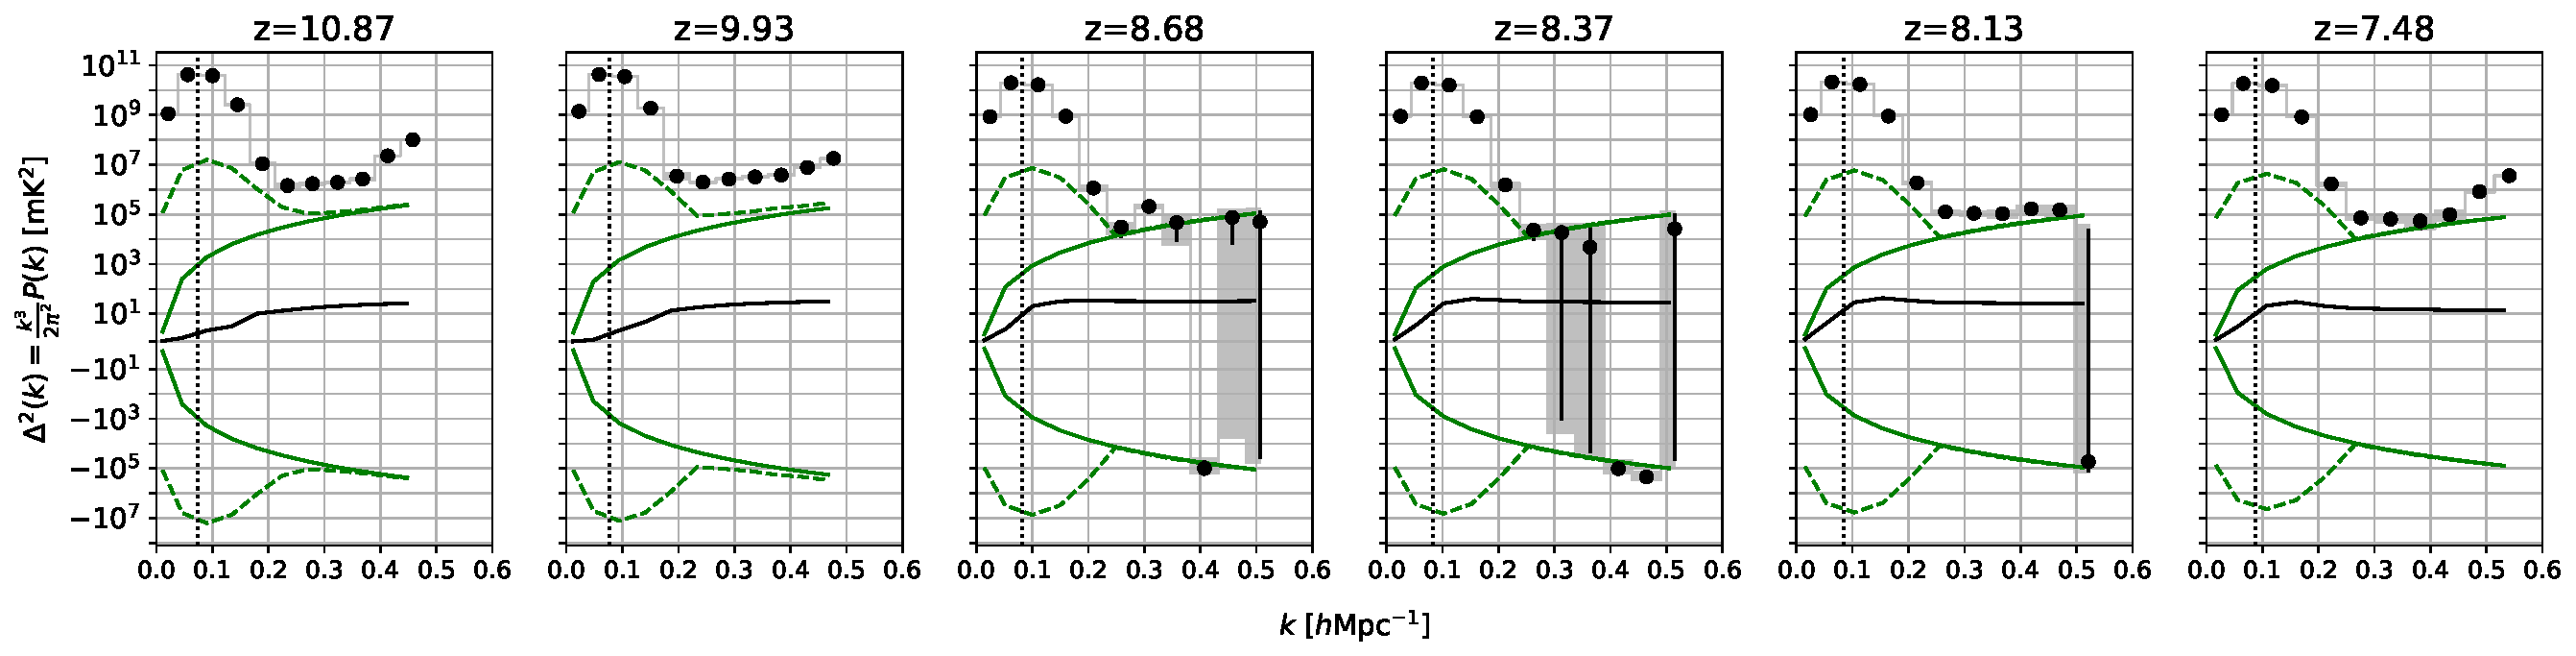
\includegraphics[width=\textwidth]{plots/pspec_flagged_ants_delta2.pdf}
\caption{The dimensionless power spectrum $\Delta^{2}(k)$ and their uncertainties derived from the PAPER-64 observations (black).
All error bars represent $ 2\sigma $ uncertainties. Also plotted are theoretical thermal noise limits estimated from Equation \eqref{eq:sense} (solid green) and a foreground-dependent variance estimate (dashed green and gray shaded; Kolopanis et al. (\textit{in prep.}).
The black solid line represents a fiducial \texttt{21cmFAST} model of reionization.
The horizon line (vertical dotted black) has been transformed from the maximum
signal delay between antennas to cosmological co-moving scales using Equations 12 and 13  of \citet{liu_et_al2014a}. }
\label{fig:pspec_delta2}
\end{figure*}

 \begin{figure*}[tp]
\centering
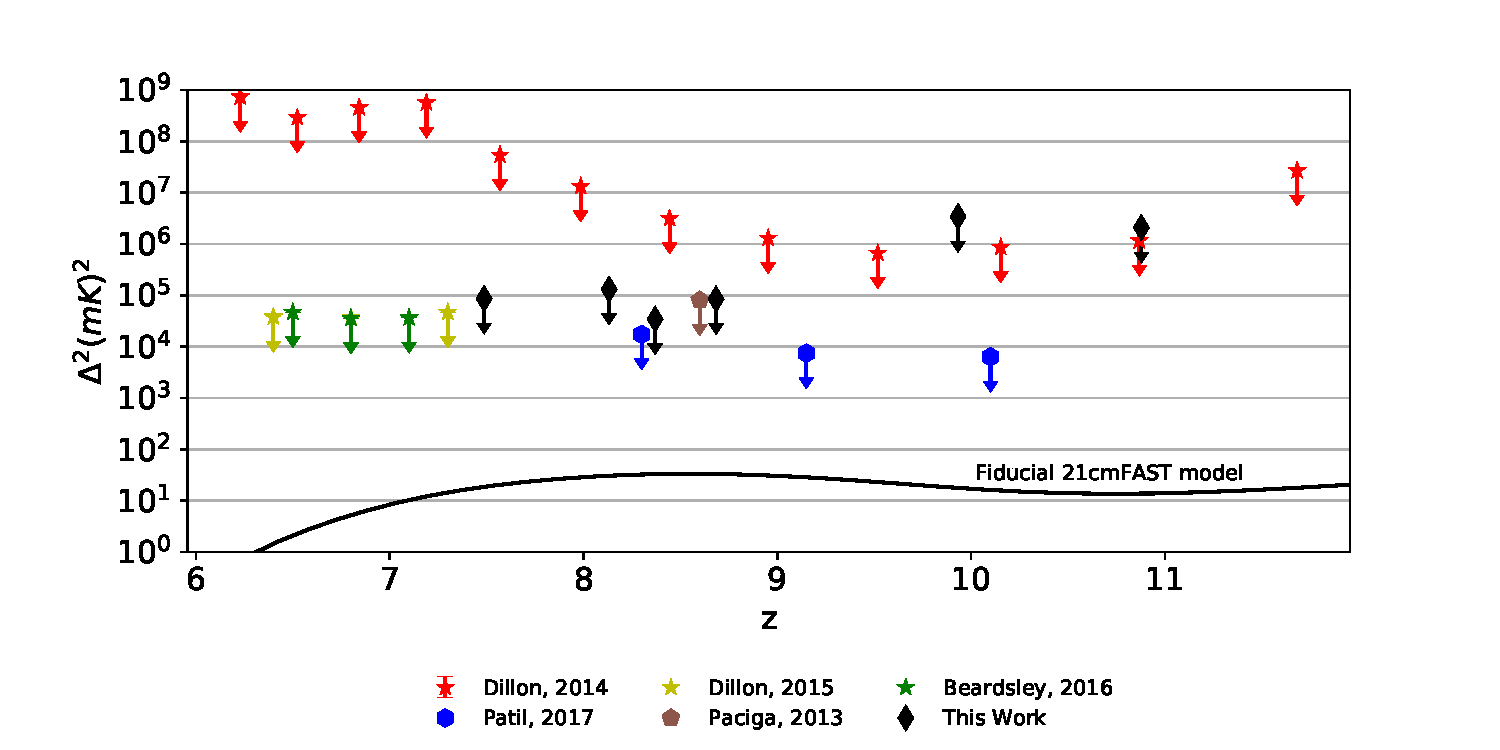
\includegraphics[width=.95\textwidth]{plots/eor_lowest_limits.pdf}
\caption{A comparison of the lowest limits achieved by various instruments in the $k$-ranges reported by each instrument.
The results reported here are taken in the range
$.3 \leq k \leq .6\ \hMpci$. Data is taken
from the MWA (stars; \cite{dillon_et_al2013b,dillon_et_al2015,beardsley_et_al2016}),
the GMRT (pentagon; \cite{paciga_et_al2013}),
LOFAR (hexagons; \cite{patil_et_al2017}),
and PAPER (diamonds; this work).
We include the $z=8.37$ redshift bin analyzed in \citet{ali_et_al2015}, although
it is worth noting this redshift bin is not entirely independent
from the $z=8.13$ and $8.68$ bins, as can be inferred from the
overlapping window functions from Figure~\ref{fig:freq_select}.
For reasons described throughout this thesis,
these PAPER results supersede all previous PAPER limits.
\label{fig:eor_summary}}
\end{figure*}

In conclusion, we have re-analyzed the PAPER-64 data first presented in \citetalias{ali_et_al2015},
 and presented 21\,cm
power spectra and uncertainties in five independent (six total) redshift bins. These estimates
are made using an independently developed pipeline
which skips foreground subtraction and simplifies time-averaging. Simulations
of noise and foregrounds are used to build a basic picture of
internal consistency. The resulting power spectra are consistent with noise
across much of the spectrum, but above redshift $9$ (below $130$\,MHz) they demonstrate
a statistically significant excess of power. Null-tests support a picture where
power spectrum detections are caused by foregrounds modulated by
spectrally dependent deviations from redundancy or calibration error.
In particular, the z-scores and imaginary power tests suggest that residuals
could be the result of some net non-redundant signal
or imperfections in baseline placement at the
$ \sim 1\% $ level for the $ 30 $~m baselines
analyzed in this work.

Future analyses of highly redundant sky
measurements will require strict comparisons
between nominally redundant samples before
cross-multiplication to ensure effects like
these can be mitigated. Also, further jackknives
and comparisons of data should be performed before or as part of LST-binning
to detect likely contributions to excess.
Precise antenna placement will also be required
to ensure baselines designed to be redundant do not
introduce signal in the imaginary component of the power spectrum.

To date, as shown in Figure~\ref{fig:eor_summary}, all power spectrum estimates have been reported as
upper limits. However, to discern and characterize the physics
of reionization, high significance detections of the 21\,cm power
spectrum are necessary.
Next generation radio telescopes,
like the fully realized 350 element configuration of HERA
\citep{pober_et_al2014,deboer_et_al2017,liu_parsons_2016}
and the
future Square Kilometre Array (SKA; \citet{mellema:2013}), are predicted to
be able to make these detections and place stringent constraints
on reionization.



